\documentclass[12pt]{article}
\usepackage[top=1in, bottom=1in, left=1in, right=1in]{geometry}
%\usepackage[margin=1in]{geometry}
\usepackage[onehalfspacing]{setspace}
%\usepackage[doublespacing]{setspace}
\usepackage{amsmath, amssymb, amsthm}
\usepackage{enumerate, enumitem}
\usepackage{fancyhdr, graphicx, proof, comment, multicol}
\usepackage[none]{hyphenat} % This command prevents hyphenation of words
\binoppenalty=\maxdimen % This command and the next prevent in-line equation breaks
\relpenalty=\maxdimen
%    Good website with common symbols
% http://www.artofproblemsolving.com/wiki/index.php/LaTeX%3ASymbols
%    How to change enumeration using enumitem package
% http://tex.stackexchange.com/questions/129951/enumerate-tag-using-the-alphabet-instead-of-numbers
%    Quick post on headers
% http://timmurphy.org/2010/08/07/headers-and-footers-in-latex-using-fancyhdr/
%    Info on alignat
% http://tex.stackexchange.com/questions/229799/align-words-next-to-the-numbering
% http://tex.stackexchange.com/questions/43102/how-to-subtract-two-equations
%    Text align left-center-right
% http://tex.stackexchange.com/questions/55472/how-to-make-text-aligned-left-center-right-in-the-same-line
\usepackage{microtype} % Modifies spacing between letters and words
\usepackage{mathpazo} % Modifies font. Optional package.
\usepackage{mdframed} % Required for boxed problems.
\usepackage{parskip} % Left justifies new paragraphs.
\linespread{1.1} 


%figure support
\usepackage{import}
\usepackage{xifthen}
\pdfminorversion=7
\usepackage{pdfpages}
\usepackage{transparent}
\newcommand{\incfig}[1]{%
	\def\svgwidth{\columnwidth}
	\import{./figures/}{#1.pdf_tex}
}
\graphicspath{ {./figures/} }
\pdfsuppresswarningpagegroup=1

\newenvironment{problem}[1]
{\begin{mdframed}[linewidth=0.8pt]
        \textsc{Problem #1:}

}
    {\end{mdframed}}

\newenvironment{solution}
    {\textsc{Solution:}\\}
    {\newpage}% puts a new page after the solution
    
\newenvironment{statement}[1]
{\begin{mdframed}[linewidth=0.6pt]
        \textsc{Statement #1:}

}
    {\end{mdframed}}

%\newenvironment{prf}
 %   {\textsc{Proof:}\\}
 %   {\newpage}% puts a new page after the solution

\begin{document}
% This is the Header
% Make sure you update this information!!!!
\noindent
\textbf{CNT3004.01} \hfill \textbf{Brandon Thompson} \\
\normalsize Prof. Ding \hfill Due Date: -- \\

% This is where you name your homework
\begin{center}
\textbf{Notes Chapter 4}
\end{center}
	\section{Overview Of Network Layer}
	The network layer forwards packets from the routers input to the appropriate router output. The route packets take is determined by the routing algorithm of the router.
	\subsection{Data Plane}
	Data plane is a local function in the router responsible for determining how a datagram arriving on an input port is forwarded to an output port.
	\subsection{Control Plane}
	Control plane is network-wide logic that determines the route a datagram will take between routers from a source host to a destination host.\\
	The control plane can be managed either by traditional routing algorithms (in the routers), or software-defined networking, SDN (remote servers).
	\section{What's inside a router}
	In a high level overview, routers contain input ports, routing processor, switching fabric, and output ports. The software in the routing processor (control plane) operates in millisecond time frame, and the forwarding process (data plane) operates in nanosecond time frame.

	Input ports should lookup the output port using a forwarding table, the goal is to complete this at ''line speed,'' and queue datagrams if they arrive faster than forwarding rate.

	Input ports can forward datagrams using destination-based forwarding, using only the destination IP address (traditional), or generalized forwarding which uses any header field values. 
	\subsection{Destination-Based Forwarding}
	\begin{center}
		\begin{tabular}{|l|c|}
			\hline
			\textbf{Destination address range} & Link interface\\
			\hline
			11001000 00010111 00010000 00000000 & \\through & 0\\11001000 00010111 00010111 11111111 & \\
			\hline
			11001000 00010111 00011000 00000000 & \\
			through & 1\\
			11001000 00010111 00011000 11111111 & \\
			\hline
			11001000 00010111 00011001 00000000 & \\
			through & 2\\
			11001000 00010111 00011111 11111111 & \\
			\hline
			otherwise & 3\\
			\hline
		\end{tabular}
	\end{center}
	\subsection{Longest Prefix Matching}
	\begin{center}
		\begin{tabular}{|l|c|}
			\hline
			\textbf{Destination Address Range} & Link interface\\
			\hline
			11001000 00010111 00010*** ******** & 0\\
			\hline 
			11001000 00010111 00011000 ******** & 1\\
			\hline
			11001000 00010111 00011*** ******** & 2\\
			\hline
			otherwise & 3\\
			\hline
		\end{tabular}
	\end{center}
	\subsection{Switching Fabrics}
	The switching fabric is responsible for transferring the packet from the input buffer to the correct output buffer. The speed of the switching fabric is called the switching rate: the rate packets can be transferred from the input to the output. Switching rate is measured as multiple of input/output line rate. $N$ inputs: switching rate = $N \times $ line rate desirable.

	There are three types of switching fabrics, memory, bus, and crossbar.
	\subsubsection{Switching via Memory}
	This method was used by first generation routers switching packets under direct control of the CPU. Speed was limited by memory bandwidth.
	\begin{figure}[ht!]
		\centering
		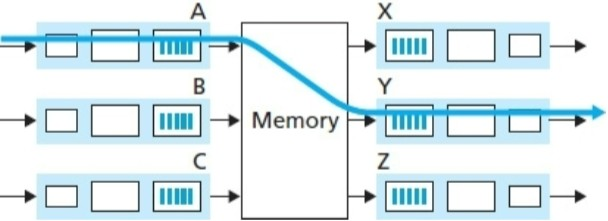
\includegraphics[width=0.8\textwidth]{mem_swt}
		\caption{Diagram of memory based switching fabric.}
		\label{fig:mem_swt}
	\end{figure}
	\subsubsection{Switching via Bus}
	Much better option over the memory switching, removes a internal storage component. Switching speed is limited by the bus bandwidth, called bus contention.
	\begin{figure}[ht!]
		\centering
		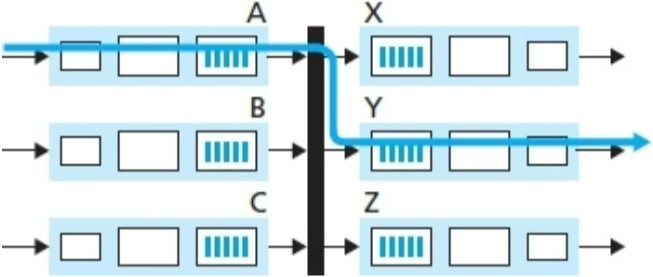
\includegraphics[width=0.8\textwidth]{bus_swt}
		\caption{Diagram of bus switching fabric.}
		\label{fig:bus_swt}
	\end{figure}
	\subsubsection{Switching via Crossbar}
	Crossbar switching is an improvement on the bus switching fabric, removes the bus bandwidth limit.
	\begin{figure}[ht!]
		\centering
		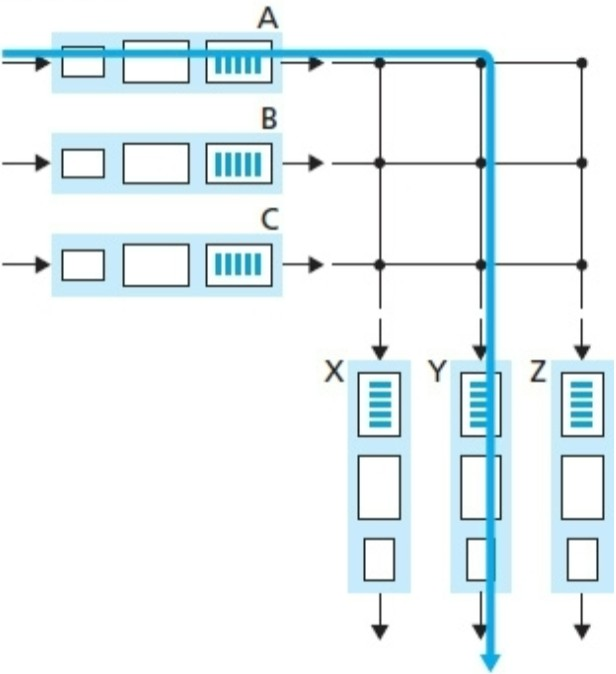
\includegraphics[width=0.8\textwidth]{cross_swt}
		\caption{Diagram of crossbar switching fabric.}
		\label{fig:cross_swt}
	\end{figure}
\end{document}
